

\chapter{This is the first chapter} \label{cha:Optimierung}
asdasad
\section{this is the first section}
\label{sec:firstsections}
asdasdadasd
\section{this is the second section}
\label{sec:secondsections}
all god stuff of the first section can be found at \secref{sec:firstsection}
\subsection{what a great subsection}
asdasd \footnote{Kapitel 4 in \cite{Farhat1991}}
as
da\\
asd
\cite{Optimierung2012}\\
asdasd \cite{Farhat1998}


\begin{equation} \label{eq:test}
    \begin{aligned} 
        AAAAAAAAAAAAA &= AAAAA\\
        B &= BBBBBBBBBBBBBBBB\\
        C &= CCCCC, D=DDDDDDD\\    
        E &= EEEEE, F=FFFFFFF
    \end{aligned}
\end{equation}



\begin{figure}[h!]
	\begin{center}
	    \fbox{\subimport{./}{fig/tikz/setup_quad4_basic_example.tex}}
        %\documentclass{standalone}
\usepackage{tikz}
\usetikzlibrary{positioning}
\begin{document}
\begin{tikzpicture}
		\def\subsize{2}%
		\def\sep{1.0}    %separation between rectangles
%		subsize
%		\draw[black, thick] ( \sep, \sep) rectangle ( \sep+\subsize, \sep+\subsize);
%		\draw[black, thick] (-\sep, \sep) rectangle (-\sep-\subsize, \sep+\subsize);
%		\draw[black, thick] (-\sep,-\sep) rectangle (-\sep-\subsize,-\sep-\subsize);
%		\draw[black, thick] ( \sep,-\sep) rectangle ( \sep+\subsize,-\sep-\subsize);

       %define nodes
       \node (N1) at (-\subsize,-\subsize)  {};%{N1};
       \node (N2) at (0        ,-\subsize)  {};%{N1};
       \node (N3) at (+\subsize,-\subsize)  {};%{N1};
       \node (N4) at (-\subsize,0)          {};%{N1};
       \node (N5) at (0        ,0)          {};%{N1};
       \node (N6) at (+\subsize,0)          {};%{N1};
       \node (N7) at (-\subsize,\subsize)   {};%{N1};
       \node (N8) at (0        ,\subsize)   {};%{N1};
       \node (N9) at (+\subsize,\subsize)   {};%{N1};
       
       \draw[fill=lightgrey,thick] (N1) rectangle (N5);
       \draw[fill=lightgrey,thick] (N2) rectangle (N6);
       \draw[fill=lightgrey,thick] (N4) rectangle (N8);
       \draw[fill=lightgrey,thick] (N5) rectangle (N9);
       
       \node[draw, circle, fill=white, font=\small]  at (N1) {1};
       \node[draw, circle, fill=white, font=\small]  at (N2) {2};
       \node[draw, circle, fill=white, font=\small]  at (N3) {3};
       \node[draw, circle, fill=white, font=\small]  at (N4) {4};
       \node[draw, circle, fill=white, font=\small]  at (N5) {5};
       \node[draw, circle, fill=white, font=\small]  at (N6) {6};
       \node[draw, circle, fill=white, font=\small]  at (N7) {7};
       \node[draw, circle, fill=white, font=\small]  at (N8) {8};
       \node[draw, circle, fill=white, font=\small]  at (N9) {9};


        % nodes
       \node (N11) at (-\sep-\subsize,+\sep)          {};%{N11};
       
       \node (N12) at (-\sep         ,+\sep)          {};%{N12};
       \node (N13) at (-\sep         ,+\sep+\subsize) {};%{N13};
       \node (N14) at (-\sep-\subsize,+\sep+\subsize) {};%{N14};
       
       \node (N21) at (+\sep         ,+\sep          ){};%{N21};
       \node (N22) at (+\sep+\subsize,+\sep          ){};%{N22};
       \node (N23) at (+\sep+\subsize,+\sep+\subsize) {};%{N23};
       \node (N24) at (+\sep         ,+\sep+\subsize) {};%{N24};
       
       \node (N31) at (+\sep,-\sep-\subsize)          {};%{N31};
       \node (N32) at (+\sep+\subsize,-\sep-\subsize) {};%{N32};
       \node (N33) at (+\sep+\subsize,-\sep)          {};%{N33};
       \node (N34) at (+\sep,-\sep)                   {};%{N34};
       
       \node (N41) at (-\sep-\subsize,-\sep-\subsize) {};%{N41};
       \node (N42) at (-\sep,-\sep-\subsize)          {};%{N42};
       \node (N43) at (-\sep,-\sep)                   {};%{N43};
       \node (N44) at (-\sep-\subsize,-\sep)          {};%{N44};
       
       
		
		
		\end{tikzpicture}
		\begin{tikzpicture}
		
		%\definecolor{fillcolor}{RGB}{200,200,200}
       \draw[fill=lightgrey,thick] (N11) rectangle (N13);
       \draw[fill=lightgrey,thick] (N21) rectangle (N23);
       \draw[fill=lightgrey,thick] (N31) rectangle (N33);
       \draw[fill=lightgrey,thick] (N41) rectangle (N43);
       
       %lagrange multipliers
       \draw[<->] (N12) edge (N21) node [fill=white, font=\small] at ($(N12)!0.5!(N21)$) {\framebox{$_2^1$}};
       \draw[<->] (N13) edge (N24) node [fill=white, font=\small] at ($(N13)!0.5!(N24)$) {\framebox{$_4^3$}};
       \draw[<->] (N12) edge (N34) node [fill=white, font=\small] at ($(N12)!0.35!(N34)$) {\framebox{$_6^5$}};
       \draw[<->] (N11) edge (N44) node [fill=white, font=\small] at ($(N11)!0.5!(N44)$) {\framebox{$_8^7$}};
       \draw[<->] (N12) edge (N43) node [fill=white, font=\small] at ($(N12)!0.5!(N43)$) {\framebox{$_{10}^9$}};
       \draw[<->] (N21) edge (N34) node [fill=white, font=\small] at ($(N21)!0.5!(N34)$) {\framebox{$_{12}^{11}$}};
       \draw[<->] (N22) edge (N33) node [fill=white, font=\small] at ($(N22)!0.5!(N33)$) {\framebox{$_{14}^{13}$}};
       \draw[<->] (N21) edge (N43) node [fill=white, font=\small] at ($(N21)!0.35!(N43)$) {\framebox{$_{16}^{15}$}};
       \draw[<->] (N31) edge (N42) node [fill=white, font=\small] at ($(N31)!0.5!(N42)$) {\framebox{$_{18}^{17}$}};   
       \draw[<->] (N34) edge (N43) node [fill=white, font=\small] at ($(N34)!0.5!(N43)$) {\framebox{$_{20}^{19}$}};
       
       
       % doflabels
       \node[anchor=south west]  at (N11) {$_{8}^{7}$};%{N11};
       \node[anchor=south east]  at (N12) {$_{10}^{9}$};%{N12};
       \node[anchor=north east]  at (N13) {$_{16}^{15}$};%{N13};
       \node[anchor=north west]  at (N14) {$_{14}^{13}$};%{N14};
       
       \node[anchor=south west]  at (N21) {$_{10}^{9}$};%{N21};
       \node[anchor=south east]  at (N22) {$_{12}^{11}$};%{N22};
       \node[anchor=north east]  at (N23) {$_{18}^{17}$};%{N23};
       \node[anchor=north west]  at (N24) {$_{15}^{16}$};%{N24};
       
       \node[anchor=south west]  at (N31) {$_{4}^{3}$};%{N31};
       \node[anchor=south east]  at (N32) {$_{6}^{5}$};%{N32};
       \node[anchor=north east]  at (N33) {$_{12}^{11}$};%{N33};
       \node[anchor=north west]  at (N34) {$_{10}^{9}$};%{N34};
       
       \node[anchor=south west]  at (N41) {$_{2}^{1}$};%{N41};
       \node[anchor=south east]  at (N42) {$_{4}^{3}$};%{N42};
       \node[anchor=north east]  at (N43) {$_{10}^{9}$};%{N43};
       \node[anchor=north west]  at (N44) {$_{14}^{13}$};%{N44};
       %\node[circle split, draw, fill=white, font=\small] at (N44) {13 \nodepart{lower} 14};
		
		\end{tikzpicture}
		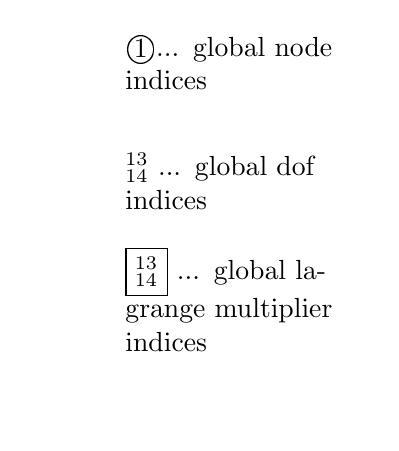
\begin{tikzpicture}
		\node[anchor=south west,text width=3cm] (I1) at (1,0) {\textcircled{\raisebox{-0.9pt}{1}}... global node indices};
		\node [anchor=south west,below of = I1,text width=3cm, node distance=1.5cm] (I2) {$_{14}^{13}$ ... global dof indices};
		\node [anchor=south west,below of = I2,text width=3cm, node distance=1.5cm] (I2) {\framebox{$_{14}^{13}$} ... global lagrange multiplier indices\\};
		\node at (0,-4) {};
		
		\end{tikzpicture}
\end{document}
	    \caption[short caption]{aaaaaaaaaaaaaaaaa}
		\label{fig:ele_setup}
    \end{center}
\end{figure}

%
\begin{figure}[h!]
	\begin{center}
	\subimport{./}{fig/tikz/setup_quad4_basic_example_sub3.tex}
    \caption[short captionaa]{aaaaasdaaaaaaaaaaaa}
		\label{fig:basic_feti_example_2x2}
    \end{center}
\end{figure}

asdasdasdad \ref{Sanders:AveragingMethods2007}\\
asdasdasd \ref{Optimierung2012}



%%%\begin{equation}
%%%\begin{array}{lc}
%%%  \texttt{$B^{(3)}=$} & \kbordermatrix{\text{}&1 &2 &3 &4 &5 &6\cr
%%%1&\0&\0&\0&\0&\0&\0\cr
%%%2&\0&\0&\0&\0&\0&\0\cr
%%%3&\0&\0&\0&\0&\0&\0\cr
%%%4&\0&\0&\0&\0&\0&\0\cr
%%%5&\0&\0&-1&\0&\0&\0\cr
%%%6&\0&\0&\0&-1&\0&\0\cr
%%%7&\0&\0&\0&\0&\0&\0\cr
%%%8&\0&\0&\0&\0&\0&\0\cr
%%%9&\0&\0&\0&\0&\0&\0\cr
%%%10&\0&\0&\0&\0&\0&\0\cr
%%%11&\0&\0&-1&\0&\0&\0\cr
%%%12&\0&\0&\0&-1&\0&\0\cr
%%%13&\0&\0&\0&\0&-1&\0\cr
%%%14&\0&\0&\0&\0&\0&-1\cr
%%%15&\0&\0&\0&\0&\0&\0\cr
%%%16&\0&\0&\0&\0&\0&\0\cr
%%%17&1&\0&\0&\0&\0&\0\cr
%%%18&\0&1&\0&\0&\0&\0\cr
%%%19&\0&\0&1&\0&\0&\0\cr
%%%20&\0&\0&\0&1&\0&\0}\\
%%%\end{array},~~
%%%\begin{array}{lc}
%%%  \texttt{$l^{(3)}=$} & \kbordermatrix{\text{}&1 &2 &3 &4 &5 &6 &7 &8\cr
%%%1&1&\0&\0&\0&\0&\0&\0&\0\cr
%%%2&\0&1&\0&\0&\0&\0&\0&\0\cr
%%%3&\0&\0&\0&\0&1&\0&\0&\0\cr
%%%4&\0&\0&\0&\0&\0&1&\0&\0\cr
%%%5&\0&\0&\0&\0&\0&\0&1&\0\cr
%%%6&\0&\0&\0&\0&\0&\0&\0&1}\\
%%%\end{array}
%%%\end{equation}


\begin{figure}[h]
\centering
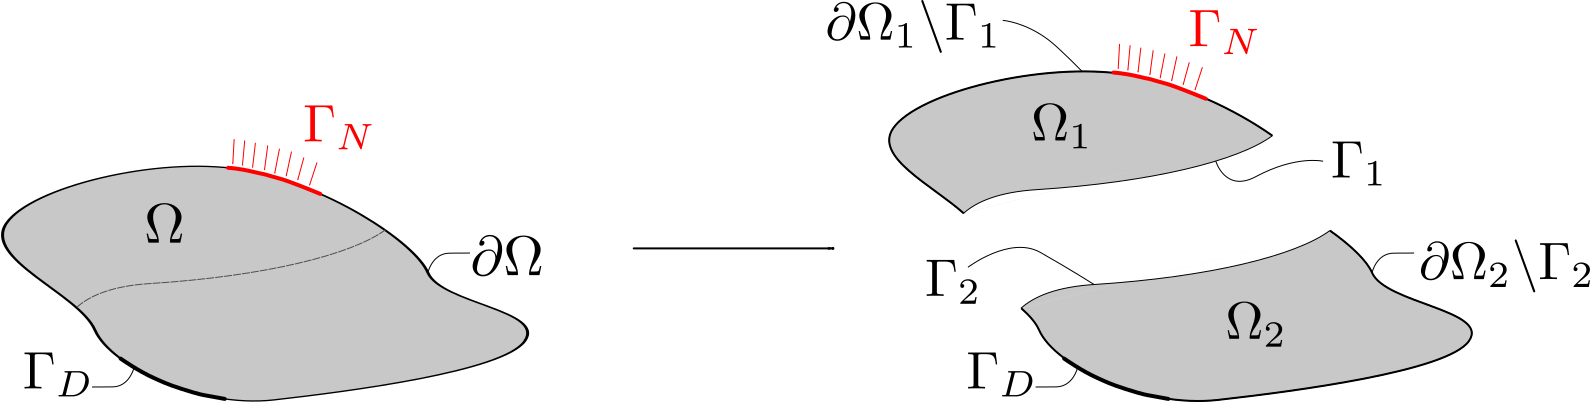
\includegraphics[width=0.8\textwidth]{./fig/eps/drawing1}
\caption[sssssssss]{adadadsada}\label{fig:reference_problem}
\end{figure}

%%%On $\Omega$:
%%%\begin{align}
%%%\dmat{K}\dvec{u}=\dvec{f}
%%%\end{align}
%%%
%%%A Lagrange multiplier approach is used two connect the two domains
%%%\begin{align}
%%%\idone{\dmat K}\idone{\dvec u}&=\idone{\dvec f}\\
%%%\idtwo{\dmat K}\idtwo{\dvec u}&=\idtwo{\dvec f}\\
%%%(\dvec{\lambda},\dvec{\idtwo u}-\dvec{\idone u})&=0\label{eq:lagmult_basic}
%%%\end{align}
%%%
%%%This can be generalized for an arbitrary number of subdomains to
%%%\begin{align}
%%%\ids{\stiffmat} \ids{\dispvec} = \ids{\dvec{f}}+{\ids{\traceop}}^T {\ids{\asmop}}^T \lagvec\label{eq:basic_subdomain_equation}\\
%%%\sum_s \ids{\traceop} \ids{\asmop} \ids{\dispvec}=0\label{eq:basic_subdomain_equation_asm}
%%%\end{align}
%%%where $\ids{\asmop}$ is a subtructure-based, boolean assembly operator, whos rows correspond to the global lagrange multipliers, and whos columns relate to the substructure-based interface-dofs. A negativ sign is used, when the lagrange multiplier connects to a substructure with a smaller ID, otherwise a positive sign is entered. This reflects the condition from Equation~\eqref{eq:lagmult_basic}.\\
%%%The trace operators $\ids{\traceop}$, map the columns of $\ids{\asmop}$ to a substructure-based total dof numbering scheme.\\
%%%For the basic example as described in Figure~\ref{fig:basic_feti_example_2x2}\\
%%%\linebreak

---------------subsection The idea of FETI\\
%%%The basic idea of FETI now is to reduce the substructure domain problems to a connected interface problem. This can be achieved very elegantly, be rearranging the basic equations REF-REF ans was first described by \ref{Farhat1991}.
%%%
%%%Equation \eqref{eq:basic_subdomain_equation} can be written as:
%%%\begin{align}
%%%\ids{\dispvec}=\inv{\ids{\stiffmat}} (\ids{\dvec{f}}+\tp{\ids{\traceop}} \tp{\ids{\asmop}} \lagvec)
%%%\end{align}
%%%
%%%Inserted into Equation~\eqref{eq:basic_subdomain_equation_asm} this gives
%%%\begin{align}
%%%&\sum_s \ids{\asmop} \ids{\traceop} \inv{\ids{\stiffmat}} (\ids{\dvec{f}}+\tp{\ids{\traceop}} \tp{\ids{\asmop}} \lagvec)=0\text{   or}\\
%%%&(\sum_s \ids{\asmop} \ids{\traceop} \inv{\ids{\stiffmat}} \tp{\ids{\traceop}}\tp{\ids{\asmop}} ) \lagvec =
%%%\sum_s \ids{\asmop}  \ids{\traceop} \inv{\ids{\stiffmat}} \ids{\forcevec}
%%%\end{align}
%%%
%%%bbbbb
%%%\begin{align}
%%%\ids{\dispvec}=\inv{\ids{\stiffmat}} (\ids{\dvec{f}}+\tp{\ids{\traceop}} \tp{\ids{\asmop}} \lagvec) + \ids{\nullspacemat} \ids{\rmodevec}
%%%\end{align}
%%%
%%%
%%%ccccc
%%%\begin{align}
%%%&\sum_s \ids{\asmop} \ids{\traceop} \inv{\ids{\stiffmat}} (\ids{\dvec{f}}+\tp{\ids{\traceop}} \tp{\ids{\asmop}} \lagvec)=0\text{   or}\\
%%%&\underbrace{(\sum_s \ids{\asmop} 
%%%\underbrace{\ids{\traceop} \inv{\ids{\stiffmat}} \tp{\ids{\traceop}}}_{\ids{\dmat{F}}}
%%%\tp{\ids{\asmop}} }_{\dmat{F}} ) \lagvec +
%%%\sum_s \underbrace{\ids{\asmop}  \ids{\traceop} \ids{\nullspacemat}}_{\ids{\rmodespace}} \ids{\rmodevec}
%%%=
%%%\underbrace{\sum_s \ids{\asmop}  \ids{\traceop} \inv{\ids{\stiffmat}}  \ids{\forcevec}}_{-\dvec{d}}
%%%\end{align}
%%%
%%%So far, the system is undertermined, since we only have two equations, but three unknowns. However, a third equation can be derived by looking at Equation~\ref{eq:basic_subdomain_equation}. If $\ids{\stiffmat}$ is singular, a solution can only exist if $\ids{\dvec{f}}+{\ids{\traceop}}^T {\ids{\asmop}}^T \lagvec$ has no component in the Nullspace $\nullspacemat$:
%%%\begin{align}
%%%&\tp{\ids{\nullspacemat}}(\ids{\dvec{f}}+{\ids{\traceop}}^T {\ids{\asmop}}^T \lagvec)=0\text{  or}\label{eq:reason_natural_subspace}\\
%%%&\underbrace{\tp{\ids{\nullspacemat}} \ids{\dvec{f}}}_{\tp{\ids{\dvec{e}}}} =
%%%\underbrace{\tp{\ids{\nullspacemat}}  \tp{\ids{\traceop}} \tp{\ids{\asmop}}}_{\tp{\ids{\rmodespace}}} \lagvec  
%%%\end{align}
%%%
%%%bla bla1
%%%\begin{align}
%%%\begin{bmatrix}
%%%\locdualschur & \rmodespace\\
%%%\tp{\rmodespace} &\dmat{0}
%%%\end{bmatrix}
%%%\begin{bmatrix}
%%%\lagvec\\
%%%\rmodevec
%%%\end{bmatrix}
%%%=
%%%\begin{bmatrix}
%%%\ifacedispvec\\
%%%\dvec{e}
%%%\end{bmatrix}
%%%\end{align}

%%%bla bla2
%%%\begin{align}
%%%\ids{\nullspacemat}&=ker(\ids{\stiffmat}) \\
%%%\end{align}
%%%
%%%bla bla3
%%%\begin{align}
%%%\dmat{e}&=\tp{\begin{bmatrix} \cdots,\tp{\ids{\forcevec}} \ids{\nullspacemat},\cdots \end{bmatrix}} \\
%%%\rmodespace&=\begin{bmatrix} \cdots,\ids{\asmop}\ids{\traceop}\ids{\nullspacemat},\cdots \end{bmatrix} \\
%%%\locdualschur&=~~\sum_s \ids{\asmop} \ids{\locdualschur} \tp{\ids{\asmop}} \\
%%%\ifacedispvec&=-\sum_s \ids{\asmop}  \ids{\traceop} \inv{\ids{\stiffmat}}  \ids{\forcevec}
%%%\end{align}


Some text is required here.
\begin{align}
\lagvec_0 &= \scalemat\rmodespace\inv{(\tp{\rmodespace}\scalemat\rmodespace)}\dvec{e} \\
\projn&=\eyemat - \scalemat\rmodespace\inv{(\tp{\rmodespace}\scalemat\rmodespace)}\tp{\rmodespace}
\end{align}

bla bla4
\begin{align}
\scaled{\locschur}=\sum_s \ids{{\scaled{\asmop}}} \ids{{\scaled{\locschur}}}
{\ids{{\scaled{\asmop}}}}{}^T  \\
\end{align}
bla bla5
\begin{align}
\tp{\projn}\locdualschur\projn\scaled{\lagvec}=\tp{\projn} (\sum_s \ids{\asmop}  )
\end{align}
bla bla6
\begin{align}
\scaled{\lagvec}_0&=\cspace\inv{(\tp{\cspace}\locdualschur\cspace)}\tp{\cspace} (\ifacedispvec-\locdualschur\lagvec_0)\\
\projc&=\eyemat-\cspace\inv{(\tp{\cspace}\locdualschur\cspace)}\tp{\cspace} \locdualschur
\end{align}


\begin{figure}[h!]
\centering
\subimport{./}{fig/tikz/algorithm_feti2.tex}
\caption[FETI-2 algorithm]{FETI-2 algorithm}
\label{diag:feti2}
\end{figure}

\begin{figure}[h!]
\centering
\subimport{./}{fig/tikz/algorithm_fetis.tex}
\caption[FETI-S algorithm]{FETI-S algorithm}
\label{diag:fetis}
\end{figure}

\begin{figure}[h!]
\centering
\subimport{./}{fig/tikz/algorithm_fetib.tex}
\caption[FETI-B algorithm]{FETI-B algorithm}
\label{diag:fetib}
\end{figure}